\documentclass{article}
\usepackage{styles/project_style}
\addbibresource{references/projects.bib}

% --- TITLE PAGE INFORMATION ---
\title{Introduction to Game Level Design by Cellular Automata}

\begin{document}
\maketitle

\section{What are Cellular Automata?}

Cellular Automata (CA) are discrete mathematical models widely used across various disciplines to simulate complex systems and emergent behaviors. A cellular automaton consists of a regular grid of cells, each in one of a finite number of states (e.g., "on" or "off," "alive" or "dead"). The grid evolves over discrete time steps according to a set of predefined rules, which determine the next state of each cell based on its current state and the states of its neighbors. These simple rules can give rise to intricate and unpredictable patterns, making CA a powerful tool for modeling phenomena in physics, biology, computer science, and beyond.

\begin{figure}[h!]
    \centering
    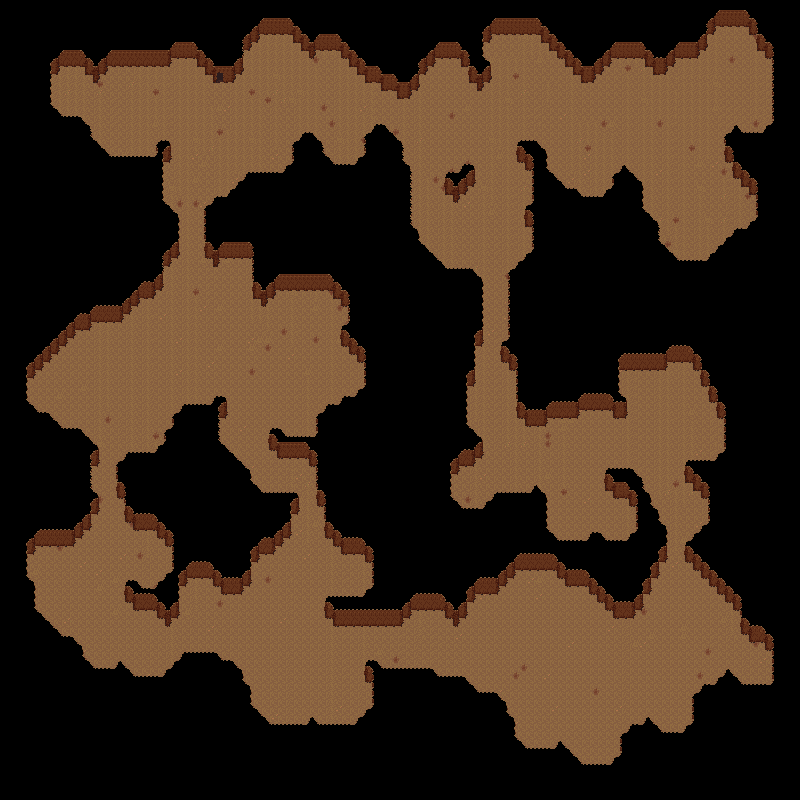
\includegraphics[width=0.35\textwidth]{projects/game_level_design/images/ca_cave.png}
    \caption{Image of procedurally generated dungeon in game Vagabond. Note that the cellular automata make only ta part of the algorithm.}
\end{figure}


Historically, cellular automata were introduced by John von Neumann and Stanislaw Ulam in the 1940s as a framework for studying self-replicating systems. The concept gained widespread recognition with John Conway's "Game of Life" in 1970, a two-dimensional CA that demonstrated how basic rules could produce complex, life-like behaviors. Today, CA are applied in diverse areas, such as simulating fluid dynamics, modeling tumor growth, and generating procedural content in computational design.

\begin{figure}[h!]
    \centering
    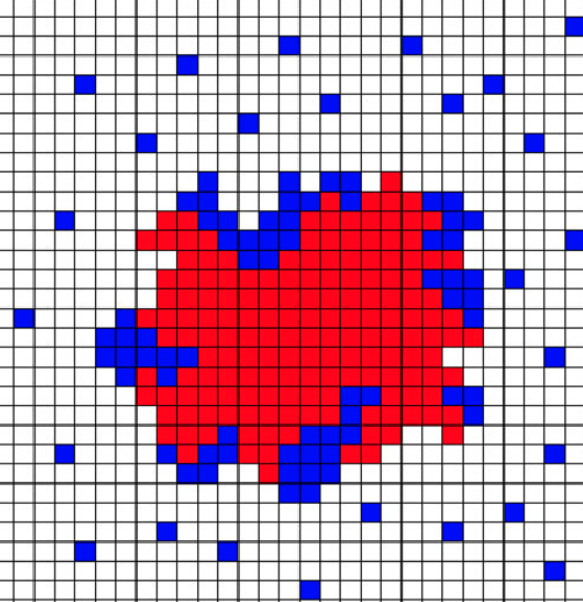
\includegraphics[width=0.35\textwidth]{projects/game_level_design/images/ca_tumor.png}
    \caption{Example of cellular automata application. The cellular automaton simulates the growth of a tumor in the presence of immune effector cells. The grid depicts tumor cells in red, immune cells in blue, and other areas occupied by healthy or dead cells. Vertical black stripes along the boundary of the square domain represent nutrient-diffusing vessels. The rest of the boundary is subject to periodic boundary conditions. Immune cells are scattered throughout the region, with some forming clusters that move and reduce the tumor size, dicussed in  \textcite{Lpez2017_game_level}}
\end{figure}


In the context of game development, cellular automata are particularly valuable for \textbf{procedural level design}. They enable developers to generate diverse and organic game environments—such as terrains, caves, or dungeons—algorithmically, rather than making each element manually. This approach not only saves time but also enhances replayability by creating unique levels for each playthrough. For instance, a CA can simulate natural processes like erosion or growth to produce realistic landscapes. 




\section{Types of Cellular Automata in Game Design}

Several types of cellular automata are commonly adapted for game level design, each suited to specific generation tasks:

\begin{itemize}
    \item \textbf{Conway's Game of Life:} A classic CA with a 2D grid where cells live, die, or reproduce based on the number of live neighbors. While not directly used in most games, its principles inspire dynamic environment simulations.
    \item \textbf{Cave Generation Automata:} These use rules to simulate erosion or geological processes, creating natural-looking cave systems with open spaces and tunnels, ideal for exploration games.
    \item \textbf{Terrain Generation Automata:} Designed to mimic natural landscape formation (e.g., mountains, rivers), these CA are widely used in open-world games to generate varied topography.
    \item \textbf{Dungeon Generation Automata:} Tailored for structured yet randomized layouts, these CA produce room-and-corridor designs for roguelike or dungeon-crawling games.
\end{itemize}

Each type can be customized by adjusting grid size, neighborhood definitions (e.g., Moore or von Neumann), and transition rules to suit a game's aesthetic and functional needs.

\section{Importance of Cellular Automata in Game Level Design}

The application of cellular automata in game level design offers significant advantages:

\begin{itemize}
    \item \textbf{Procedural Generation:} CA create unique levels each time, increasing replayability and reducing predictability.
    \item \textbf{Efficiency:} Automating level creation saves development time, allowing focus on gameplay mechanics or narrative.
    \item \textbf{Organic Complexity:} Simple rules yield intricate, natural-looking structures—like jagged caves or sprawling forests—that enhance immersion.
    \item \textbf{Flexibility:} Rules and parameters can be tweaked to match different genres, from survival games to strategy titles.
\end{itemize}

These benefits make CA an indispensable tool for modern game design, particularly in indie development and large-scale procedural worlds.

\section{Mathematical Representation}

A cellular automaton is formally defined by:

\begin{itemize}
    \item \textbf{Grid:} A lattice (typically 2D) of cells, each with a state from a finite set (e.g., $\{0, 1\}$ for empty or filled).
    \item \textbf{Neighborhood:} A set of adjacent cells influencing a given cell, such as the Moore neighborhood (8 surrounding cells) or von Neumann neighborhood (4 cardinal directions).
    \item \textbf{Transition Rules:} A function mapping the current state of a cell and its neighbors to its next state.
\end{itemize}

For example, a simple cave-generation CA might use these rules on a binary grid ($0$ = empty, $1$ = wall):
\begin{itemize}
    \item If a wall cell has fewer than 4 wall neighbors, it becomes empty (erosion).
    \item If an empty cell has more than 4 wall neighbors, it becomes a wall (sedimentation).
\end{itemize}

Mathematically, for a cell in position $(x, y)$ in grid $G_t$ at time $t$, the next state $G_{t+1}(x, y)$ is:
\[
G_{t+1}(x, y) = f(G_t(x, y), N(x, y))
\]
where $N(x, y)$ is the count of the neighborhood state and $f$ is the rule function. Iterating this process over multiple steps refines the level structure.

\section{Implementation Example}

No implementation example is given for this project, as the development of the algorithm is the main task of the project.  

\section{Literature}
\subsection{General introduction}
Good general introduction on Cellular Automata is Wikipedia. The topic of game level design well discussed in several blogs that describe game development. Here are several resources:
\begin{itemize}
    \item \href{https://en.wikipedia.org/wiki/Cellular_automaton}{Wikipedia:Cellular automaton}
    \item \href{https://medium.com/@yvanscher/cellular-automata-how-to-create-realistic-worlds-for-your-game-2a9ec35f5ba9}{Cellular Automata: How to Create Realistic Game Levels}
    \item \href{https://is.muni.cz/th/w12aw/SimulatingWorldsCA.pdf}{Simulating Game Worlds Using Cellular Automata} (a master thesis)
    \item \href{https://medium.com/nerd-for-tech/a-peek-at-cellular-automata-1-2-ee0bf60204fa}{A peek at cellular automata (1/2)}
    \item \href{https://www.jeremykun.com/2012/07/29/the-cellular-automaton-method-for-cave-generation/}{The Cellular Automaton Method for Cave Generation}
\end{itemize}


For further exploration:
\subsection{Journal Club books}
Game level design is described in several academic papers. Here are a few papers suitable for the Journal Club presentation:
\begin{itemize}
 \item \textcite{Adams2017_game_level}
 \item \textcite{Earle2022_game_level}
  \item \textcite{Johnson2010_game_level}
\item \textcite{Pech2016_game_level}
\end{itemize}



\section{Conclusion}

Cellular automata are an interesting tool for game level design.   Simple rules give rice with emergent complexity. Their ability to generate varied, organic environments improves both development efficiency and player engagement.

\printbibliography

\end{document}